\documentclass{scrreprt}
\usepackage{graphicx}
\graphicspath{ {images/} }
\usepackage{listings}
\usepackage{underscore}
\usepackage[bookmarks=true]{hyperref}
\usepackage{hyperref}
\hypersetup{
	bookmarks=false,    % show bookmarks bar?
	pdftitle={Software Requirement Specification},    % title
	pdfauthor={Christopher Silva},                     % author
	pdfsubject={TeX and LaTeX},                        % subject of the document
	pdfkeywords={TeX, LaTeX, graphics, images}, % list of keywords
	colorlinks=true,       % false: boxed links; true: colored links
	linkcolor=blue,       % color of internal links
	citecolor=black,       % color of links to bibliography
	filecolor=black,        % color of file links
	urlcolor=purple,        % color of external links
	linktoc=page            % only page is linked
}%
\author{Christopher Silva}
\date{}
\def\myversion{0.1 }
\begin{document}
	\begin{titlepage}
		\flushright
		\rule{16cm}{5pt}\vskip1cm
		\Huge{SOFTWARE REQUIREMENTS\\ SPECIFICATION}\\
		\vspace{2cm}
		for\\
		\vspace{2cm}
		CMPS 4113 - Software Engineering\\
		\vspace{2cm}
		%\LARGE{\myversion\\}
		%\vspace{2cm}
		%\LARGE{Version \myversion approved\\}
		%\vspace{2cm}
		%Prepared by Christopher Silva\\
		\vfill
		\rule{16cm}{5pt}
	\end{titlepage}
	\tableofcontents
	\chapter*{Revision History}
	February 4, 2017 Initial Draft - Christopher Silva, Anthony Enem, Nathan Durst, Da Dong, and Shujing Zhang met at the Midwestern State University Library to work on the intial draft.
%===============================================================================
	\chapter{Introduction}
	Dr. Stringfellow (hereafter referred to as the client), is interested in software that will help ensure that her computer science students are writing programs that fit her specifications. This software should calculate and display metrics about the users source code such as line of code, lines of documentation, and the ratio of the two.
	\section{Purpose}
	This document details the Project Plan for the Software Metrics Calculation System (hereafter referred to as SCMS), which the Software Engineering group ID-10-T (hereafter also referred to as the team) has devised to assist in the software development process. The plan outlines the different areas of the project that must be addressed for successful development of the software. It establishes guidelines for resources that will be used in the project, and also points out additional resources that are needed. The Project Plan shows how the team is comprised and states the means of reporting. This plan addresses some of the risks involved in the project and the steps to correct those risks, if they occur. Also, quality assurance will be mentioned, and a glossary of terms used in this document is included.
	\section{Scope}
	The client wants SMCS to quickly calculate code metrics on student source code. The client currently spends an excessive amount of time looking for issues that could be solved if students had software to point them out. The client would like SMCS to support C++ and Java source code. The client would like SMCS to be easily extensible in the future to allow for more types of metrics or languages.
	\section{Main Objective}
	The main objective of SMCS is to help first and second year computer science students become better programmers by giving them a tool that will point out some frequent simple mistakes that they make.
	\section{Overview of Document}
	The remainder of the document is intended to inform the client of the intended system. Hardware and software requirements, major users, both major and minor functions, constraints, and intended user interface are described.
%===============================================================================
	\chapter{Users}
	\section{Who are the Users?}
	The principal users of the SMCS are students taken freshmen or sophomore level computer science courses. Due to the SMCS being able to analyze only C++ and/or Java source code files, the users would also need to be familiar with the language(s) accepted by the SMCS. Other users might include upper level CS students who need some analysis on their source code written in the specified language, or professors who might want to integrate the SMCS as part of their grading system to analyze student’s source code written in programming languages accepted by SMCS.
	\section{Use Cases}
	User analyzes a source code file :
	\begin{enumerate}
		\item User double clicks the SMCS’ executable file and that launches the SMCS web interface on the computer’s default browser.
		\item User loads file(s) by clicking on an open file button and selecting file(s) from an Open file dialog OR by dragging and dropping source code file(s) onto a drag-and-drop panel on the SMCS interface.
		\item User chooses programming language of uploaded source code. file(s) in one of two ways:
		\begin{enumerate}
			\item User accepts SMCS’ automatically detected programming language from the file(s) extension.
			\item User selects file(s) extension of source code file(s) from a drop-down menu of accepted languages if automatically detected language is incorrect.
		\end{enumerate}
		\item User clicks a button for SMCS to begin source code analysis.
		\item SMCS analysis
		\begin{enumerate}
			\item Main success scenario:
			\begin{enumerate}
				\item SMCS successfully completes analysis of uploaded source code file(s).
				\item SMCS displays results from analysis of uploaded file(s) to the user
			\end{enumerate}
			\item Incorrect source code file scenario :
			\begin{enumerate}
				\item File(s) uploaded by user is not of the selected programming language. SMCS displays an error of this scenario and prompts the user to select the correct programming language.
			\end{enumerate}
		\end{enumerate}
		\item User closes the SMCS application.
	\end{enumerate}
	\begin{figure}[h]
		\caption{Use Case Diagram}
		\centering
		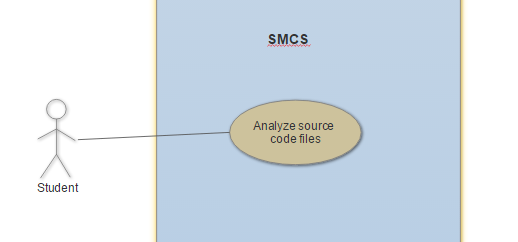
\includegraphics{use-case-diagram.png}
	\end{figure}
%===============================================================================
	\chapter{System}
	\section{Development Environment}
	The team will program SMCS in Go using JetBrains Gogland as the IDE. The team will use Git for version control, Slack for communications, and LaTeX for documentation.
	\section{Target Environment}
	SMCS must run on Windows XP or later, Linux, and Mac OS X 10.7 or later.
	\section{Functional Requirements}
	SMCS must allow the user to load a source code file and view metrics about their code. SMCS must initially support C++ and/or Java.\\
	SMCS must support the following metrics:
	\begin{itemize}
		\item Lines of Code (LOC) - The number of lines of code.
		\item Lines of Documentation (LOD) - The number of lines of documentation.
		\item Ration of LOC to LOD - This will be used to tell the user if there is too little documentation.
		\item Blank Lines - The number of blank lines. This will be used to tell a user if there is not enough whitespace.
		\item Total Lines - The total number of lines.
		\item Number of Functions - The number of functions in a file.
		\item Number of Function Parameters - The number of parameters in each function. This will be used to warn a user if there is an excessive amount of parameters in a function.
		\item Number of Non-void Functions - The number of functions that do not have a void return type.
		\item Methods Per Class - The number of methods in each class.
		\item Lines Per Function - The number of lines in each function.
		\item Cyclomatic complexity - The number of linearly independent paths within a program.
	\end{itemize}
	\section{Non-functional Requirements}
%===============================================================================
	\chapter{Risks}
	The development process of the SMCS involves several risks. All risks should be identified and action should be taken to reduce these risks to an acceptable level. Development risks include project knowledge, team member turnover, requirement adjustments, and changes in the specifications.
	\section{Possible Risks}
	The risks involved in the development of SMCS are that the developers may not have a complete understanding of the entire metric calculation system in general. Lack of experience with parsing files or using the designated programming language plays a factor in the development process. Also, the risk of team member turnover can involve a member of our team withdrawing from the course, inevitably withdrawing from the project. Additionally, the requirements set by the client can change unpredictably if the client sees issues with the current requirements of the system during the time of development. Another risk is that the client, or team, may change specifications during the development process.
	\section{Risk Managment}
	\begin{tabular}{|p{5cm}|p{9cm}|}
		\hline 
		Risk & Solution \\ 
		\hline 
		Project Knowledge &  Group meetings weekly as well as constant communication between the team using applications such as Slack and GitHub so the team is all on the same page.\\ 
		\hline 
		Team Member Turnover & Team members must discuss potential drop with the rest of the team so plans can be made.\\ 
		\hline 
		Requirements Change & Constant communication between the client and a team member to make sure that the information related to the requirements is collected accurately.\\ 
		\hline 
		Specifications Change & The client and all team members will be constantly updated on status of the project through each step of the development process. \\ 
		\hline 
	\end{tabular} 
	% add other chapters and sections to suit
\end{document}